\section{Metodologia}

Segundo \citeonline{wiltgen2019prototipos}, um protótipo é uma representação similar ao produto a ser desenvolvido, criado com o intuito de realizar testes e ensaios para que as funcionalidades se comportem como esperado no ambiente de uso. Nesse contexto, o objetivo principal deste trabalho é implementar um protótipo de um sistema VLC utilizando um SBC como plataforma de desenvolvimento. Durante o desenvolvimento foram utilizados elementos de metodologias ágeis como os do \textit{Scrum} e do \textit{Kanban}.

O \textit{Scrum} é uma estrutura que define diversos eventos como as \textit{sprints} que são ciclos de desenvolvimento com um tempo definido, geralmente de duas semanas, e a retrospectiva que é o momento em que a equipe discute o que foi bom ou ruim no ciclo (\textit{sprint}) que se passou. O \textit{Scrum} também define os membros da equipe e suas responsabilidades, como o PO, o \textit{Scrum Master} e a equipe de desenvolvimento \cite{scrum}. 

O \textit{Kanban} é uma estrutura que permite a visualização dos itens de trabalho que são organizados em um quadro que é dividido em \textit{To Do}, \textit{In Progress} e \textit{Done} \cite{kanbam}.

Para a avaliação do desempenho das SBCs selecionadas foram coletadas as informações de uso do processador, o uso de memória RAM e também a taxa de erros durante a transmissão de um pacote de dados.

\subsection{Single Board Computer (SBC)}

\textit{Single Board Computer} (SBC) é um computador onde todos os componentes necessários estão em uma mesma placa de circuito impresso. Esse tipo de dispositivo é muito utilizado para fins educacionais, para desenvolvimento de sistemas, datacenters (centros  de  processamento  de  dados) e clusters portáteis. Alguns exemplos são o \textit{OrangePI}, \textit{RockPI}, \textit{BeagleBone} e \textit{RaspberryPI}, sendo este um dos mais populares \cite{SBC_edu}.

Os SBCs geralmente são de baixo custo, porém devido a escassez global de semicondutores reduziu a sua disponibilidade e por consequência levou ao aumento dos preços \cite{zeng_2022}. Principalmente do \textit{RaspberryPI} que passou de 45 dólares para 161 dólares, por esse motivo o SBC \textit{OrangePI} foi selecionado para o desenvolvimento deste trabalho.

\subsubsection{RaspberryPI}

A \textit{Raspberry Pi Foundation} foi fundada em 2008 sediada no Reino Unido com o objetivo de promover o avanço na educação no campo da computação. \cite{rasp}

O \textit{RaspberryPI} é um pequeno computador que traz consigo um processador na arquitetura ARM, a mesma tecnologia que se encontra em num smartphone \cite{rasp}.\newline

\begin{figure}[!htbp]
  \caption{Raspberry Pi 3}
  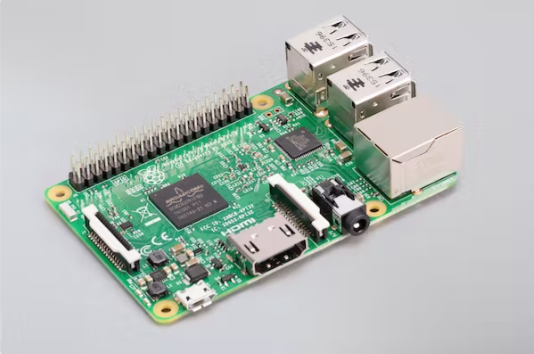
\includegraphics[scale=0.4]{images/rasp.png}
  \legend{Fonte: \citeonline{rasp}}
  \label{figura:rasp}
\end{figure}

\subsubsection{OrangePI}

O \textit{OrangePI} é um SBC \textit{open source} da Shenzhen Xunlong Software. A arquitetura de seu processador é ARM e a plataforma suporta vários sistemas operacionais como Android e as várias distribuições de linux \cite{orangepi}.\newline

\begin{figure}[!htbp]
  \caption{Orange Pi 3 LTS}
  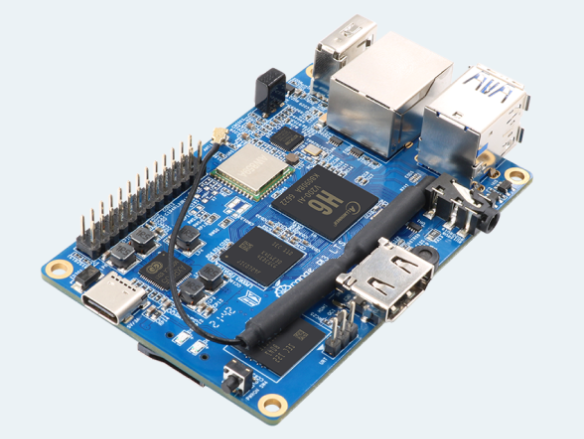
\includegraphics[scale=0.35]{images/orange.png}
  \legend{Fonte: \citeonline{orangepi}}
  \label{figura:orange}
\end{figure}

\newpage

\subsubsection{BeagleBone Black}

\textit{BeagleBone Black} é uma plataforma suportada pela comunidade que roda Linux para prototipagem rápida \cite{beaglebone}.
Esta plataforma é utilizada pelo projeto OpenVLC. \newline

\begin{figure}[!htbp]
  \caption{BeagleBone Black}
  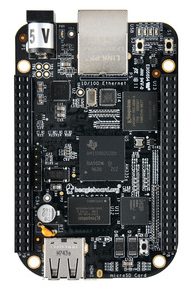
\includegraphics[scale=0.58]{images/beaglebone.png}
  \legend{Fonte: \citeonline{beaglebone}}
  \label{figura:beagle}
\end{figure}

\subsection{Linux}

Linux é um sistema operacional de computadores, o autor \citeonline{negus} cita em seu livro Linux a Bíblia que este sistema é um exemplo de como projetos colaborativos podem ultrapassar o que empresas individuais podem fazer.

O Linux permite que os desenvolvedores alterem o sistema como quiserem ajudando a criar softwares para as suas necessidades, por esse motivo utilizaremos este sistema no desenvolvimento do trabalho.
